\documentclass{article}

\usepackage[a4paper,margin=1in]{geometry}

\usepackage{hyperref}
\usepackage[utf8]{inputenc}
\usepackage[english]{babel}
\usepackage{textpos}
\usepackage{textcomp}
\usepackage{amsmath}
\usepackage{amssymb}
\usepackage{amsfonts}
\usepackage{graphicx}
\usepackage{epstopdf}
\usepackage{algorithmic}
\usepackage{verbatim}
\usepackage{textcomp}
\usepackage{varwidth}
\usepackage[linesnumbered,ruled]{algorithm2e}
\usepackage{multicol}
\usepackage{palatino}

% For displaying code
\usepackage{listings}

\usepackage{enumitem}
% Change format of top-level list items
%\setlist[enumerate,1]{label*=\arabic*,font=\bfseries,before=\bfseries}
% Reset formatting for subsequent levels; label type makes 1.1, legal-style labels
%\setlist[enumerate,2]{label*=.\arabic*,font=\normalfont,before=\normalfont}

% Theorem
\newtheorem{theorem}{Theorem}

% lists
\usepackage{outlines}
\usepackage{enumitem}
\newenvironment{tight_enum}{
\begin{enumerate}[label=\alph*.]
\setlength{\itemsep}{0pt}
\setlength{\parskip}{0pt}
}{\end{enumerate}}

% \subsubsubsection{}
\setcounter{secnumdepth}{5}
\setcounter{tocdepth}{5}
\newcommand\simpleparagraph[1]{%
  \stepcounter{paragraph}\paragraph*{\theparagraph\quad{}#1}}

\usepackage{color}
\usepackage{xcolor}
\usepackage{mdframed}

\definecolor{dkgreen}{rgb}{0,0.6,0}
\definecolor{gray}{rgb}{0.5,0.5,0.5}
\definecolor{mauve}{rgb}{0.58,0,0.82}

% \usepackage{courier}
\lstset{%frame=tb,
language=C++,
aboveskip=3mm,
belowskip=3mm,
showstringspaces=false,
columns=flexible,
basicstyle={\small\ttfamily},
numbers=none,
numberstyle=\tiny\color{gray},
keywordstyle=\color{blue},
commentstyle=\color{dkgreen},
stringstyle=\color{mauve},
breaklines=true,
breakatwhitespace=true,
tabsize=3
}

%%%%%%%%% BEGIN DOCUMENT %%%%%%%%%
%%%%%%%%% BEGIN DOCUMENT %%%%%%%%%
%%%%%%%%% BEGIN DOCUMENT %%%%%%%%%

%% Used tt when referring to function

\begin{document}

\title{Engineerging Programming II: \\ Monte Carlo Simulation}
\author{Graham West}
\date{}

\maketitle

\large

\tableofcontents


%%%%%%%%%%%%%
%%% NEW SECTION %%%
%%%%%%%%%%%%%
\section{Intro to MC}

Suppose you have a random variable $x \sim p(x)$ ($x$ is drawn from $p$) and that you want to compute any of the following:
\begin{enumerate}
	\item The distribution of $f(x)$
	\item The mean of $f$ over $p$: $\int f(x) p(x) dx$
\end{enumerate}
These quantities can be very challenging to compute analytically if $f,p$ have complex analytical forms. Worse, they can be impossible if $f,p$ do not even have analytical forms. Fortunately, they can be solved via \emph{Monte Carlo Simulation} or (Monte Carlo Sampling). Monte Carlo methods are a class of methods which utilize random sampling from a probability distribution in order to solve problems which would be very difficult or impossible via other analytical means.

Take the first problem for instance: finding the distribution of $f(x)$ where $x \sim p(x)$. There are analytical techniques to find the distribution of a function of a random variable, but they are usually restricted to certain types of functions or distributions and can be very difficult to perform. If an analytical form is not necessary, we can simply use a monte Carlo approach:
\begin{enumerate}
	\item Draw $N$ random samples of $x \sim p(x)$:
			\\ $x^i, i = 1, \cdots N$
	\item Evaluate $f(x)$ for each of these samples:
			\\ $f(x^i) = f^i, i = 1, \cdots N$
\end{enumerate}
You now have $N$ random samples ($f^i$) from the distribution of $f(x)$.

Take the second problem: finding the mean of $f$ over $p$: $\int f(x) p(x) dx$. Well, having found the distribution of $f(x)$ in the previous problem, we can approximate the mean $\hat f$ of the $f^i$:
\begin{equation}
	\hat f = \frac{1}{N} \sum_{i=1}^N f^i
\end{equation}
Now this is only the sample mean of $f$, not the population mean (which would be given by the integral above). However, according to the strong law of large numbers, the sample mean approachs the population mean as the number of samples grows larger:
\begin{equation}
	\lim_{N\rightarrow\infty} \frac{1}{N} \sum_{i=1}^N f^i = \int f(x) p(x) dx
\end{equation}
Also, the standard deviation $\sigma(\hat f)$ of the sample mean decreases as number of samples decreases.

In summary, using a computer to draw a large number of samples from a distribution and then evaluating some function of them is much easier than complex analytical methods.


%%%%%%%%%%%%%
%%% NEW SECTION %%%
%%%%%%%%%%%%%
\section{Calculating $\pi$ and integrals}

\subsection{Calculating $\pi$}

We can use Monte Carlo methods to calculate the value of $\pi$. Consider the unit circle inscribed in a square. We can compute the areas of the two figures:
\begin{enumerate}
	\item Circle: $A_C = \pi r^2 = \pi \cdot 1^2 = \pi$
	\item Square: $A_S = s^2 = 2^2 = 4$
\end{enumerate}
\begin{figure}[h]
	\centering
	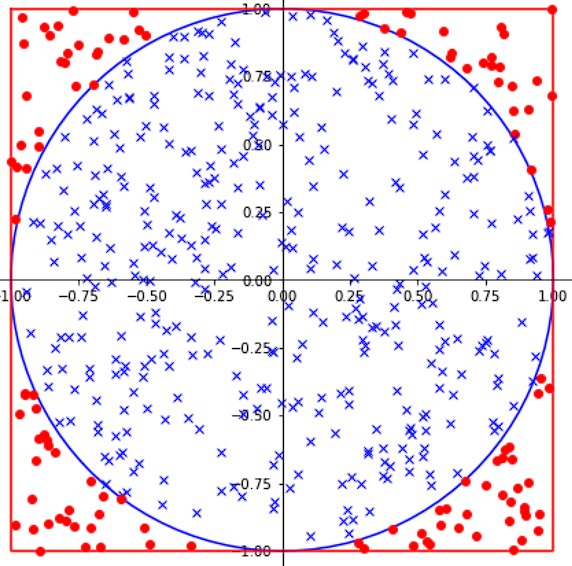
\includegraphics[width=0.5\linewidth]{CircleSquare_Points}
	\caption{A circle inscribed in a square with randomly generated points.}
\end{figure}
We can compute the ratio of the areas: $A_C/A_S = \pi/4$. Now, this ratio also represents the fraction of the square's area which the circle takes up. We can get an estimate of this fraction by generating a large number $N$ of points within the square and determining what fraction of them also lie within the circle $N_C/N$. In accord with the law of large numbers,
\begin{equation}
	\lim_{N\rightarrow\infty} N_C/N = A_C/A_S
\end{equation}
So, we cacn approximate $\pi = 4 A_C/A_S \approx 4 N_C/N$ with increasing accuracy as we choose larger and larger $N$. Thus, we have used a Monte Carlo method to estimate the value of $\pi$.


\subsection{Evaluating integrals}

We can use a similar approach as that above to evaluate complex integrals. Suppose we wish to evaluate
\begin{equation}
	\int_{-1}^{2} e^{-x^2} \textrm{sin}^2(4\pi x) dx
\end{equation}
Like with the circle, we can inscribe a plot of this function in a rectangle with $x$ bounds that match the integral limits ([-1,2]) and $y$ bound which enclose the entire range of values (we chose [-0,1.5]). (NOTE that the $y$ bound DO NOT have to be the maximum and minimum of the function.)
\begin{figure}[h]
	\centering
	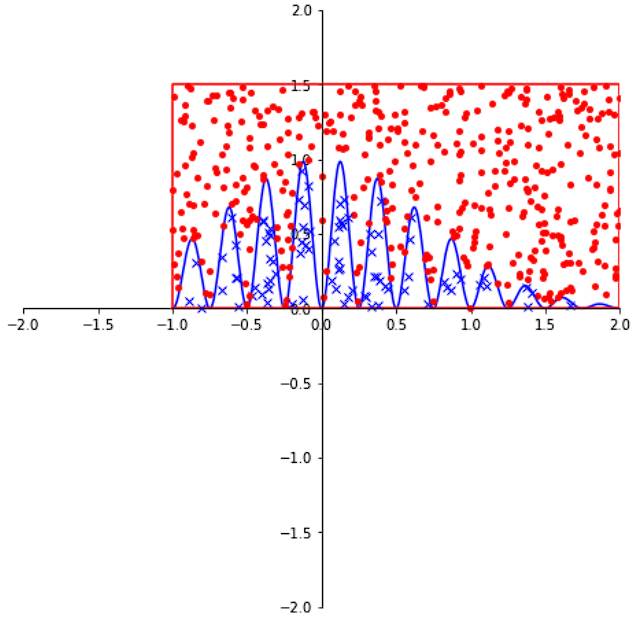
\includegraphics[width=0.5\linewidth]{Integral_Points}
	\caption{Integrating a function with Monte Carlo.}
\end{figure}
Now, we can randomly sample $N$ points inside the rectanlge and check what fraction of them lie below the graph of the function. Thus, letting $A_{rect}$ equal the area of the rectangle and $A_{int}$ equal the area under the curve (i.e., the value of the integral), we have
\begin{equation}
	\int_{-1}^{2} e^{-x^2} \textrm{sin}^2(4\pi x) dx = A_{int} = A_{int} \frac{A_{rect}}{A_{rect}} = \frac{A_{int}}{A_{rect}} A_{rect} \approx \frac{N_{int}}{N} A_{rect}
\end{equation}
where $N_{int}$ is the number of points which lie below the function. As before, this approximation becomes more accurate as $N$ increases.


%%%%%%%%%%%%%
%%% NEW SECTION %%%
%%%%%%%%%%%%%
\section{Homework}

\subsection{Birthday Paradox}

The birthday paradox is a common problem in probability theory. It concerns calculating the probability that---in a group of $N$ people---at least two individuals will share a birthday. Particularly, the probability of a shared birthday exceeds 50\% in a group of only 23 people.

Use MC sampling to generate a graph showing the probability of shared birthdays. Also, derive a formula for the probability and plot it on the same graph (with a legend). Do the graphs seem to agree?

\subsection{Integrating sin$(x)$}

Use MC sampling to show (approximate) that $\int_{-\pi}^{\pi} \textrm{sin}(x) dx = 0$. (NOTE: you will have to do a bit of extra work on top of the usual MC integration to account for the negative values of sin$(x)$.)

\subsection{2D Integral}

Use MC sampling to evaluate the 2D integra
\begin{equation}
	\int \int_{D} \frac{1}{2 \pi} \textrm{exp}(-(x^2+y^2)/2) dA
\end{equation}
where $D$ is a circle of radius 3, centered on $(1,-1/2)$.



\end{document}
